% Alternative preprint version — full demonstration-suite resource paper.
% Not tied to a specific venue's template (arXiv doesn't require one); plain
% article class. Differs from the two venue-specific drafts in this repo:
%   - papers/nature-communications/  -> strict NC structure, VVIQ16-scale
%     empirical framing, sn-jnl (Springer Nature) class.
%   - papers/neurips-neuroai/        -> 5pp, interpretability-only (demos
%     05/06), NeurIPS workshop template.
%   - THIS FILE                      -> broader resource paper, framework +
%     all six examples/demonstration\_suite/0X_*/ modules as Results, no page limit.
% Companion D&B-track submission (psychscanner_neurips/) covers framework +
% VVIQ16 only; this preprint is the version with the full demo suite.

\documentclass[11pt]{article}
\usepackage[utf8]{inputenc}
\usepackage[T1]{fontenc}
\usepackage[margin=1in]{geometry}
\usepackage{amsmath,amssymb}
\usepackage{hyperref}
\usepackage{graphicx}
\usepackage{booktabs}
\usepackage{natbib}
\usepackage{pifont}
\newcommand{\xmark}{\ding{55}}

\title{Beyond predictive benchmarks: infrastructure for hypothesis-driven cognitive testing of large language models}

% Names, order, and affiliations verified directly from the title page of
% arXiv:2607.29093 (metasignal, same author team minus Odegaard) — quoted
% verbatim, not inferred. Corresponding author email matches CITATION.cff.
\author{%
  Saurabh Ranjan\thanks{Corresponding author: \texttt{ranjan.saurabh@outlook.com}} \\ \small University of Florida
  \and
  Konstantina Sokratous \\ \small University of Missouri
  \and
  Mukesh Makwana \\ \small Brown University
}
\date{}

\begin{document}
\maketitle

\begin{abstract}
Large language models are increasingly studied as psychological subjects,
but the communities doing so apply incompatible standards of evidence:
NeuroAI evaluates a model by how well it predicts responses to naturalistic
stimuli, while psychology evaluates it by how well it accounts for the
effect of manipulating a controlled stimulus to test a falsifiable,
mechanism-level hypothesis. Running the second kind of study at the scale
quantitative psychology expects currently has no dedicated infrastructure:
prompt construction, response parsing, memory management, persona
conditioning, and feedback injection are hand-built for every new task and
model family. We present \textbf{psychscanner}, an open-source framework in
which a researcher authors a controlled cognitive or survey task once, as a
declarative task card, and runs it across memory architectures, persona
manipulations, feedback regimes, agent architectures, and model families
without rewriting the underlying mechanics. We describe the framework's
architecture and report a six-module demonstration suite exercising its
feature surface on real model calls. Two modules have complete data. A
three-armed bandit task run through three agent architectures found none
produced explore-then-exploit behaviour, and that the dominant effect was
instruction-following collapse under structured feedback rather than an
architecture difference. A 480-trial factorial replication of a classic
imagery paradigm found no measurable effect of persona conditioning on
vividness ratings, but that single-turn prompting returned an identical
rating on all 160 of its trials --- a response-degeneracy artifact
invisible to any aggregate score. Because every model backend implements
one interface, the same task cards additionally capture residual-stream
activations, which we validate by reproducing the Othello-GPT board-state
probing result on a toy transformer trained for the purpose. In both
completed behavioural demonstrations the informative result sat one level
below the headline metric and became visible only because the design varied
one factor at a time.
\end{abstract}

\section{Introduction}

Large language models are increasingly treated as objects of psychological
inquiry in their own right \citep{hagendorff2023machinepsych,
binz2023gpt3cogpsy} — evaluated for their memory, personality self-report,
imagery, and reasoning much as a human participant would be. But the
research communities doing this evaluation do not share a common
methodology, and the resulting disagreements are not merely about findings;
they are about what counts as evidence in the first place. NeuroAI
typically evaluates a model by how well it predicts behavioural and neural
responses to naturalistic stimuli, treating out-of-sample predictive
variance on broad benchmarks as the mark of success and alignment with
biological computation as the underlying goal \citep{binz2025foundation}.
Psychology, by contrast, evaluates a model by how well it accounts for the
effect of systematically manipulating a controlled, artificial stimulus —
changing one factor at a time to test a specific, falsifiable hypothesis
about a specific mechanism \citep{bowers2023deepproblems}. These are not
interchangeable standards: a model can predict naturalistic behavioural
data well while getting the underlying mechanism wrong, and a model
narrowly tuned to a controlled manipulation may generalize poorly to
naturalistic settings. Recent work has made this tension explicit as a
live methodological disagreement rather than a settled question, with
researchers reaching opposite conclusions about how much NeuroAI's
predictive successes actually tell us about biological
intelligence.\footnote{See the 2026 Cognitive Computational Neuroscience
(CCN) Generative Adversarial Collaboration organized by Jeffrey Bowers and
colleagues, ``Is NeuroAI adopting the right methods and theoretical
frameworks to advance our understanding of mind and brain?''
\citep{gac2026neuroai}, whose kickoff workshop set Milton Montero
(current NeuroAI methods are problematic) against Martin Schrimpf (current
methods are appropriate), with Jenelle Feather and Anya Ivanova arguing a
middle position. The GAC's own proposal frames the disagreement across
five methodological axes: the goal and scope of modelling, whether
engineering success is a valid starting point, whether naturalistic or
controlled stimuli are the right evaluation target, how a model should be
evaluated (predictive variance vs.\ manipulation-driven effect sizes), and
the role of falsification.}

This disagreement is not abstract, and it is not confined to vision models.
In a June 2026 preprint, Bowers and colleagues make the general critique
concrete against a large language model: they argue that Centaur
\citep{binz2025foundation}, fine-tuned to predict human trial-by-trial
responses across a large database of psychology experiments, is not subject
to the cognitive constraints it is meant to model, that its behaviour is
better characterised as role-play than as a mechanistic account, and more
generally that predictive power is being mistaken for explanatory power
\citep{bowers2026centaurcritique}. The GAC's own comment thread reproduces
the disagreement in real time and narrows it to something closer to a
resolvable empirical question. Responding to Bowers's opening challenge —
what have we learned about mind and brain from correlational studies with
ANNs? — Michael Tarr argues that the relevant distinction is not whether a
study is correlational but whether a model comparison is
\emph{theoretically diagnostic}, and that NeuroAI already runs
manipulation-based science, just inside the model's architecture and
training rather than on its input, pointing to convergent food-selectivity
findings in ventral visual cortex across independent studies using
different ANN-guided methods as an example of what this approach has
taught us. Bowers's reply narrows the disagreement to a concrete result:
manipulating the images behind a widely used behavioural benchmark
collapses a leading brain-similarity metric's prediction accuracy from near
100\% to under 20\%, which he reads as evidence that predictive success is
often driven by shortcuts rather than shared mechanism
\citep{gac2026discussion}. Both positions concede the same limit. Tarr's
own defence of NeuroAI treats manipulating a model's assumptions as the
diagnostic move; and Bowers's closing position in the thread is explicitly
not to abandon ANNs but to ``complement this new approach with old
fashioned methods'' \citep{gac2026discussion} — systematic experimental
manipulation, at scale, which is exactly the missing infrastructure this
paper builds for large language models. Psychology's own history is a
warning against settling for the alternative: more than five decades before
this GAC, Newell argued that testing isolated hypotheses about the mind one
at a time, without shared infrastructure for accumulating results across
many controlled studies into a working theory, could not by itself add up
to psychology of the kind that explains cognition rather than merely
describing pieces of it \citep{newell1973twentyquestions}. psychscanner is
an attempt to give hypothesis-driven, manipulation-based testing of LLMs
that shared, reusable infrastructure, at the exact moment this
methodological choice is being litigated in public rather than assumed.

Applying psychology's side of this methodology to LLMs at any scale —
systematically manipulating one factor (memory architecture, persona,
feedback, stimulus modality) across many models, many replications, and
many controlled task variants, the way a human cognitive psychology lab
would run a study — has no dedicated infrastructure. A researcher wanting
to ask a falsifiable, mechanism-level question (e.g.\ does giving a model
conversational memory change how consistently it reports a stable
personality across a survey, the way it would for a human respondent?) has
to hand-write the experiment scaffolding — prompt construction, response
parsing, memory/state management, persona conditioning, feedback injection
— from scratch for every new task and every new model family, which is
exactly the kind of ad hoc, one-off tooling that makes systematic,
multi-condition, multi-model replication impractical.

We introduce \textbf{psychscanner}, an open-source framework that closes
this infrastructure gap: it lets a researcher author a controlled cognitive
or survey task once, as a declarative task card, and run it across
memory conditions, persona manipulations, feedback regimes, and model
families without rewriting any of the underlying mechanics. This is not a
benchmark and not a claim that models are or are not human-like — it is
the missing methodological toolkit for asking the kind of manipulation-based,
falsifiable question that psychology's half of the NeuroAI/psychology
divide calls for, applied to LLMs specifically, at the scale quantitative
psychology expects.

\section{Background and related work}
\label{sec:related}

\paragraph{Behavioural machine psychology.} Framing LLMs as experimental
subjects has produced evidence of human-like cognitive biases and
persona-contingent behaviour shifts
\citep{hagendorff2023machinepsych,binz2023gpt3cogpsy}, and the methodology
for doing so is now being formalized explicitly \citep{lin2025simulators}.
Benchmarks such as PsychoBench \citep{huang2024psychobench} and task
ontologies such as the Cognitive Atlas \citep{poldrack2011cogatlas} give
this approach structure and coverage targets. What they share is a limit
rather than a flaw: they characterize what a model does, and none is
designed to ask why a given response pattern occurred. Two studies run on
earlier versions of the framework described here sit squarely inside that
limit. The first found that LLM source-monitoring accuracy --- distinguishing
self-generated from externally-provided content --- degrades under
conversational delay in a pattern that tracks active rather than aggregate
parameter count, producing feedback-induced failure modes invisible to
existing benchmarks \citep{ranjan2026reality}. The second found that LLM
imagination-vividness ratings produce a degenerate, single-cluster network
topology (median ARI $\approx 0$) where three geographically distinct human
populations show robust, replicable community structure
($r = 0.31$--$0.93$) \citep{ranjan2025psychological}. Both are behavioural
results whose mechanism is unknown.

\paragraph{Neuroscience-inspired interpretability.} The methods that could
answer the second question have direct neuroscience analogues, which is
what makes the pairing natural rather than opportunistic. Linear probing
for task-relevant internal state is methodologically the same operation as
neural decoding from recorded population activity; its most visible
language-model instance is the Othello-GPT result that a transformer
trained only on legal-move sequences develops a linearly-decodable internal
board representation \citep{li2023othello}. Causal tracing and rank-one
model editing (ROME) localize and manipulate where a factual association is
stored \citep{meng2022rome}, functionally analogous to lesion and
reversible-inactivation methodology in systems neuroscience.
Contrast-Consistent Search (CCS) recovers a linear ``truth direction'' from
unlabeled activations by enforcing logical consistency between a statement
and its negation \citep{burns2023ccs}. Persona vectors
\citep{chen2025personavectors} apply the same probing and steering toolkit
to character traits such as sycophancy and hallucination propensity,
extracted from natural-language trait descriptions and monitored or
controlled at inference and fine-tuning time --- activation steering being
the analogue of stimulation along an identified pathway. psychscanner's
interpretability backend (\S\ref{sec:interp-backend}) is designed to run all
four method families through one experimental harness, on top of the same
persona and task-card system already validated for behavioural work. We
regard putting these methods inside a reusable experimental framework,
rather than leaving them as one-off analysis scripts, as a contribution in
its own right: it makes the mechanistic toolkit available on the same
platform that produced the behavioural questions in the first place.

\paragraph{Why behavioural and mechanistic testing belong in one harness.}
Interpretability research has itself recently moved toward the conclusion
that motivates keeping these two kinds of testing together rather than
treating the mechanistic side as a self-sufficient replacement for
behavioural measurement. DeepMind's mechanistic interpretability team has
argued for grounding the field in a pragmatic proxy task and starting from
the simplest method that could work, citing disappointment with the
progress delivered by ambitious reverse-engineering of model internals
\citep{nanda2025pragmatic}. A concurrent clinical-triage study makes the
resulting gap concrete: linear probes recovered hazardous cases from
internal activations at 98.2\% AUROC, yet steering on those same
directions corrected only 20\% of the errors the model's output actually
made, and disrupted 53\% of the cases it was already getting right
\citep{basu2026actionability} --- near-perfect internal representations
that none of four steering and probing methods could reliably turn into
corrected behaviour. Read together, these results say that internal state
is a complement to behavioural measurement, not a substitute for it, which
is why psychscanner's interpretability backend sits behind the same
model-provider seam as its behavioural task cards rather than as a
separate analysis pipeline. Even inside interpretability the organizing
vocabulary is borrowed from cognitive psychology: a recent survey of
attention-head function proposes a four-stage framework modelled
explicitly on the human thought process --- knowledge recalling,
in-context identification, latent reasoning, and expression preparation
--- to categorize what different attention heads do
\citep{zheng2025attentionheads}. That a psychological stage model is doing
organizing work inside mechanistic interpretability is itself a data point
for the pairing this paper argues for: the two literatures are already
asking about the same stages of processing, from different kinds of data.

\section{Framework overview}

Figure~\ref{fig:blueprint} gives the component structure of the released
package (v0.3.0). Every run traverses the same spine. The researcher's
task card and persona files are resolved into an \texttt{ExpCard}, which is
expanded into one system message per design cell and one message per trial;
\texttt{TaskRunner} executes those trials against a configured agent; and
the results are validated and written to disk as one record per
participant, exported on demand to a tidy one-row-per-trial table. Around
that spine sit four seams the researcher is expected to extend --- response
parsers, model providers, agent architectures, and trial-level feedback ---
and it is the model-provider seam that carries the interpretability
backends (\S\ref{sec:interp-backend}). The design principle throughout is
that anything a psychologist would want to manipulate as an experimental
factor should be a declaration on the card, not a code path; the
subsections below describe each part in those terms.

\begin{figure}[h]
\centering
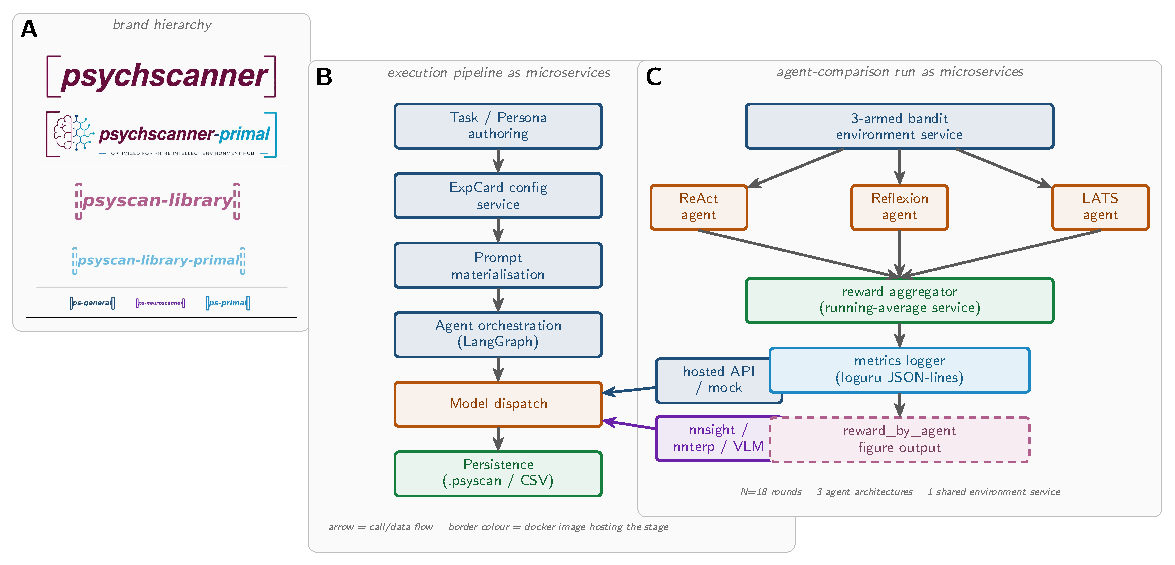
\includegraphics[width=\textwidth]{../figures/figure1_composite.pdf}
\caption{The PsychScanner project as a microservices system. (A) Brand
hierarchy: the two framework repositories (psychscanner,
psychscanner-primal), their companion vetted task/experiment-card
libraries (psyscan-library, psyscan-library-primal), and the three
published Docker images (\texttt{ps-general}, \texttt{ps-neuroscanner},
\texttt{ps-primal}). (B) The single-run execution pipeline, redrawn as a
service pipeline; box border colour marks which Docker image hosts each
stage. (C) The multi-agent bandit comparison behind
Fig.~\ref{fig:bandit}, redrawn the same way: one shared environment
service, three interchangeable agent services, and a
reward-aggregation/logging path terminating in that figure.}
\label{fig:composite}
\end{figure}

\begin{figure}[p]
\centering
\includegraphics[height=0.92\textheight,width=\textwidth,keepaspectratio]{../figures/psychscanner_blueprint.pdf}
\caption{Component blueprint of psychscanner v0.3.0. Blue marks the core
execution path traversed by every run; orange dashed boxes mark the four
researcher-facing extension seams; purple marks the interpretability
backends, which reach the rest of the framework through the same
\texttt{BaseChatModel} interface as every hosted-API backend; green marks
on-disk artifacts. Every label in the diagram is a symbol in the released
package.}
\label{fig:blueprint}
\end{figure}

\subsection{Task cards}
\label{sec:taskcards}

The unit a researcher actually authors is a \emph{task card}: a plain JSON
document (or an equivalent inline Python dict) declaring an experiment's
instructions, its named contexts, and its trials, with no code required for
the common case. Each trial carries a unique \texttt{trcode} and a stimulus
— plain text, a structured dict, or a list of multimodal content blocks
(image/audio/text) for vision-language tasks. The text before the first
underscore in a trial's \texttt{trcode} is matched against the card's
\texttt{contexts\_id} list to derive a \texttt{context\_item}: the full-text
description of whichever condition that trial belongs to. This is computed
once at prompt-build time and attached to every trial automatically, for
both prompting (when \texttt{context\_present} is set) and for output
records — an author writes the context-to-condition mapping once, rather
than repeating context text on every trial.

A single \texttt{chain\_type} field, independent of which memory mode
(stateless \texttt{SingleTurn} or continuous \texttt{Convo}) is active,
controls how trials share conversational state: \texttt{item} sends each
stimulus as an independent model call; \texttt{trial} groups the multiple
stimuli under one \texttt{trcode} into a single conversational thread (e.g.\
a study phase immediately followed by its matching test phase); \texttt{task}
places every trial for the whole run on one continuous thread. This one
parameter is what lets a single trial-execution engine implement
single-turn, trial-chain, and episodic-chain designs — the three trial
structures demonstrated across Demos 2 and 3
(\S\ref{sec:demo02}--\S\ref{sec:demo03}) and the extended factorial suite in
Supplementary Information Sections S1--S2 — without separate code paths
for each. Structured response parsing (a Pydantic schema per trial or per
card, resolved by name or passed directly), a per-trial subset of the
card's bound tools, and trial-level feedback injection (fed back into the
next trial's prompt) are declared the same way, as optional fields on the
same card, so a researcher varying these as experimental conditions edits
one card rather than one code path per condition.

\subsection{Persona conditioning and memory conditions}
\label{sec:personamemory}

Persona conditioning is authored as one or more JSON files, each holding a
list of persona statements. At prompt-build time the framework takes the
Cartesian product across those files and emits one system message per
resulting cell, so a design crossing two persona files with two levels each
yields four conditions without the researcher enumerating them by hand;
this is the machinery the WEIRD / non-WEIRD manipulations in
\S\ref{sec:demo03} and Supplementary Information S1 are built from.

Memory is configured independently of persona. \texttt{SingleTurn} compiles
the execution graph without a conversation checkpointer; \texttt{Convo}
compiles it with one. Windowing and summarization are then orthogonal
parameters rather than additional modes: \texttt{memory\_k} bounds how much
history is retained, and \texttt{summary\_k} folds the overflow into a
rolling summary prepended to the system message. Four commonly-reported
memory architectures --- stateless, unbounded conversation, windowed
conversation, and windowed rolling summary --- are therefore two parameter
settings rather than four implementations, which is what makes memory
crossable with persona and feedback inside a single factorial design
(\S\ref{sec:demo03}).

\subsection{Agent architectures and feedback}
\label{sec:agentsfeedback}

The component that executes a trial is swapped through one
\texttt{custom\_agent=} argument, against a small protocol the framework
only ever calls two members of. Alongside a bare single-call baseline, the
package ships ReAct, supervisor, planner--executor, and three reflection
variants (basic reflection, Reflexion, and LATS). Because they sit behind
the same protocol, agent architecture becomes a manipulable factor in an
otherwise identical design --- which is exactly what \S\ref{sec:demo01}
exploits.

Trial-level feedback is supplied by subclassing a single abstract class
with one method, which receives the trial and the parsed response and
returns a string; the framework folds that string into the \emph{next}
trial's prompt, handling the multimodal case as well as plain text. The
package deliberately ships no concrete feedback subclasses: reward,
correctness, and value-tracking feedback are experiment-local definitions,
because what counts as feedback is part of the experimental design rather
than the infrastructure.

\subsection{Model providers and the interpretability backend}
\label{sec:interp-backend}

Every model backend is reached through a single dispatch function and
implements the same LangChain \texttt{BaseChatModel} interface, so which
model executes a trial is a field on the \texttt{ExpCard} rather than a code
path. Hosted APIs (OpenAI, Anthropic, Groq, Ollama, OpenRouter), a
deterministic mock model for offline testing, and three local backends
built on \texttt{nnsight} are all interchangeable at that one seam.

The local backends are what make mechanistic work possible without a
parallel pipeline. \texttt{ChatNNsightModel} wraps a local Hugging Face
model and captures activations from a researcher-specified list of dotted
module paths; \texttt{ChatNNterpModel} wraps a standardized transformer
interface and addresses activations by layer index crossed with kind
(layer, attention, or MLP output) instead, which is the more convenient
addressing scheme when the same probe is to be run across model families;
and a vision-language variant extends the same capture to multimodal
prompts. Each call runs a cached forward pass over the prompt and writes
the captured per-module residual-stream activations to disk, referencing
the file from the returned message rather than embedding tensors in it ---
mirroring how the framework externalizes multimodal stimuli.

Two consequences are worth stating explicitly. First, because this sits
behind the ordinary model-provider interface, every existing mechanism ---
persona conditioning, memory modes, task cards, feedback hooks --- applies
unchanged: a persona-contrast experiment that would previously have
yielded only behavioural response differences now also yields paired
activation captures, with no separate extraction pipeline to write.
Second, capture is over the prompt's forward pass and not per generated
token, which bounds what can legitimately be asked of the resulting
tensors and is a real limitation of the current implementation rather than
a configuration detail.

\subsection{Outputs and reproducibility}
\label{sec:outputs}

Each participant's trials are validated against a nested Pydantic schema
and written as a single record; multimodal stimuli are externalized to a
content-addressed media store, so a run's outputs contain hashes rather
than repeated base64 blobs. A separate export step flattens those records
into a tidy one-row-per-trial table carrying the condition labels
(\texttt{memory}, \texttt{chain\_type}, \texttt{context\_item},
\texttt{trcode}, and the parsed response fields) alongside the raw
response, so the analysis step is an ordinary dataframe operation. A
session tunnel logs checkpoints throughout, so an interrupted
multi-participant run resumes at the last completed simulation rather than
restarting --- a practical requirement for the multi-hundred-trial,
rate-limited runs these designs produce. The full configuration
round-trips to JSON, so a run is describable by one file plus the task
card.

\subsection{Comparison with related frameworks}
\label{sec:framework-compare}

Table~\ref{tab:framework-compare} places psychscanner against six
frameworks a reader might otherwise reach for. Three are the accuracy-first
evaluation harnesses already discussed in \S\ref{sec:related}: the
EleutherAI \texttt{lm-evaluation-harness} \citep{sutawika2025evalharness},
BIG-bench \citep{srivastava2023bigbench}, and the AISI Inspect framework
\citep{aisi2024inspect}. The other two, AutoRA and SweetBean, come from a
closely related but distinct tradition: Sebastian Musslick's lab builds
tooling for closed-loop behavioural-science automation rather than
LLM-as-participant cognitive testing specifically. AutoRA automates the
scientific-discovery loop itself --- an experimentalist proposes conditions,
an experiment runner collects data (from human participants via Prolific,
a synthetic/equation experiment, or another runner), and a theorist fits a
model, with the cycle repeating \citep{musslick2024autora}; it has no
concept of a persona, a conversational LLM participant, or a task card, and
is not a fit for the same job psychscanner does. SweetBean is the closer
comparison: a declarative Python DSL that compiles one experiment
specification into either a jsPsych timeline for human participants or a
text-based prompt sequence for an LLM ``synthetic participant''
\citep{strittmatter2025sweetbean}, and explicitly interoperates with
AutoRA for closed-loop deployment. Ratings below for AutoRA and SweetBean
are drawn from their public documentation, JOSS papers, and source
(\texttt{github.com/AutoResearch/\{autora,sweetbean\}}, accessed
2026-08-13) using the same three-level scale as the original comparison:
SweetBean ships a first-class \texttt{Feedback} stimulus for trial-by-trial
correctness feedback and reinforcement, and its response specifications
carry explicit \texttt{correct\_*} fields, so it scores accuracy natively
--- stronger than psychscanner's own ``Partial'' rating on that row.
Persona conditioning in SweetBean is a single \texttt{demographic(age,
gender)} prompt template rather than an arbitrary persona-statement system;
we rate that Partial. Neither AutoRA nor SweetBean documents a dedicated
crash-safe checkpoint/resume subsystem for long API sweeps comparable to
\texttt{SessionTunnel}.

\begin{table}[h]
\centering
\caption{Feature comparison of LLM/behavioural evaluation frameworks.
\checkmark{} = first-class support; ``Partial'' = limited or requires a
workaround; \xmark{} = not supported. psychscanner, Eval Harness, Inspect,
and BIG-bench ratings are based on public documentation and source code
\citep{sutawika2025evalharness,srivastava2023bigbench,aisi2024inspect}.
AutoRA and SweetBean ratings are based on their JOSS papers and public
source \citep{musslick2024autora,strittmatter2025sweetbean}, accessed
2026-08-13.}
\label{tab:framework-compare}
\small
\begin{tabular}{@{}lccccccc@{}}
\toprule
Feature & psychscanner & Eval Harness & Inspect & BIG-bench & AutoRA & SweetBean \\
\midrule
Persona conditioning & \checkmark & Partial & \checkmark & Partial & \xmark & Partial \\
Within-session memory modes & \checkmark & Partial & \checkmark & Partial & \xmark & Partial \\
Trial-level feedback & \checkmark & \xmark & \checkmark & \xmark & \xmark & \checkmark \\
Session resume / checkpoints & \checkmark & Partial & Partial & \xmark & Partial & \xmark \\
Structured response schemas & \checkmark & Partial & Partial & \xmark & \xmark & Partial \\
Portable experiment config & \checkmark & \xmark & \xmark & \checkmark & Partial & Partial \\
JSON task specification & \checkmark & \checkmark & \checkmark & \checkmark & \xmark & Partial \\
Accuracy benchmarking & Partial & \checkmark & \checkmark & \checkmark & \xmark & \checkmark \\
\bottomrule
\end{tabular}
\end{table}

The comparison sharpens rather than flattens psychscanner's positioning.
Against the accuracy harnesses, its primary differentiators remain
structured typed response schemas enforced at the model level, memory
modes mapped directly onto between-/within-subjects designs, per-trial
adaptive feedback hooks, and portable experiment serialization
(\texttt{save\_expcard}/\texttt{load\_expcard}). Against AutoRA, the two
frameworks are complementary rather than competing: AutoRA's
experimentalist/theorist loop is a natural consumer of psychscanner-style
task cards as an \texttt{experiment\_runner}, a direction we flag as future
work rather than a present capability. Against SweetBean, the comparison is
closer and genuinely double-edged --- SweetBean's native accuracy scoring
and first-class feedback stimulus are real strengths psychscanner lacks in
equal form, while psychscanner's persona-file system, three explicit memory
architectures, and typed per-task response parsing go further than
SweetBean's single-dimension demographic prompting and general-purpose
response specs built for jsPsych's input types rather than free-form model
output.

\section{Results}
\label{sec:results}

Six demonstration modules (\texttt{examples/demonstration\_suite/01\_reward\_task} through
\texttt{06\_advanced\_demonstration}) exercise psychscanner's feature surface
end-to-end on real model calls; each is summarized below from its own
\texttt{reports/report.md}, generated directly from the run that produced it
(no numbers in this section are estimated or reused across demos).
Table~\ref{tab:demo-overview} summarizes the design and current data-collection
status of all six before the per-demo detail that follows.

\begin{table}[h]
\centering
\caption{Demonstration-suite design overview. Status reflects data
collection as of this draft, not design completeness — all six task cards,
memory/persona/feedback conditions, and analysis scripts are implemented
regardless of how much data has been collected against them.}
\label{tab:demo-overview}
\small
\begin{tabular}{@{}p{0.06\textwidth}p{0.22\textwidth}p{0.28\textwidth}p{0.2\textwidth}p{0.16\textwidth}@{}}
\toprule
Demo & Task & Key conditions & Model(s) & Data status \\
\midrule
01 & 3-armed bandit & 3 agent architectures & \texttt{llama-3.1-8b-instant} (Groq) & Complete, analyzed \\
02 & PAL-50 & single-turn / trial-chain / episodic-chain $\times$ feedback & TBD & Not started \\
03 & BFI-44 survey & 2 persona $\times$ 4 memory & \texttt{llama-3.3-70b-versatile} (Groq) & 1/8 cells \\
04 & Shape-naming VQA & 2 memory $\times$ 2 feedback & \texttt{gemma-4-26b-a4b-it:free} (OpenRouter) & 1/4 conditions \\
05 & Persona-vector probing & trait extraction/steering & \texttt{gpt2}/\texttt{gpt2-medium} & Not started \\
06 & Othello/ROME/CCS & 3 toy reproductions & toy transformer (CPU) & 1/3 (Othello only, \S\ref{sec:demo06}) \\
\bottomrule
\end{tabular}
\end{table}

\subsection{Demo 01: Agent-architecture swapping on a reward-learning task}
\label{sec:demo01}

A 3-armed bandit task (hidden reward means 2.0/6.0/4.0, value-tracking
feedback fed back each round) was run through three structurally different
\texttt{psychscanner.agents} implementations --- a bare single-call baseline
(\texttt{CustomAgent}), a generate/reflect self-critique loop, and a
plan/execute/validate loop --- plugged into the identical
\texttt{ExpCard}/\texttt{ScannerModel}/\texttt{FeedbackBase} pipeline via a
single \texttt{custom\_agent=} argument, on \texttt{llama-3.1-8b-instant}
(Groq), 6 rounds $\times$ 1 participant per agent (18 scored rounds total,
real API calls, no mocking).

None of the three architectures produced textbook explore-then-exploit
behavior: the baseline accumulated 16.14 total reward (mean 2.69/round, 0\%
optimal-arm picks), self-reflection 14.14 (mean 2.36/round, 16.7\% optimal,
the only agent to reach the optimal arm at all), and plan/execute/validate
12.14 (mean 2.02/round, 0\% optimal; Table~\ref{tab:bandit}). All three
under-selected the optimal arm (true mean 6.0) in favor of the worst arm
(true mean 2.0), and none approached the optimal arm's mean over the course
of the run (Fig.~\ref{fig:bandit}).

\begin{figure}[h]
\centering

\includegraphics[width=0.75\textwidth]{../figures/reward_by_agent.png}
\caption{Running average reward by agent architecture across the 3-armed
bandit task (Demo 01). The optimal arm's true mean (6.0) is shown as a
dashed reference line.}
\label{fig:bandit}
\end{figure}

\begin{table}[h]
\centering
\caption{Demo 01 per-agent summary. $N=18$ rounds total (6 rounds
$\times$ 3 architectures), demonstration-scale, not a powered study.}
\label{tab:bandit}
\begin{tabular}{@{}lccc@{}}
\toprule
Agent architecture & Total reward & Mean reward/round & \% optimal-arm picks \\
\midrule
Baseline (single-call) & 16.14 & 2.69 & 0\% \\
Self-reflection & 14.14 & 2.36 & 16.7\% \\
Plan/execute/validate & 12.14 & 2.02 & 0\% \\
\bottomrule
\end{tabular}
\end{table}

More important than the reward gap itself is a confound the report flags
plainly: from round 2 onward, once JSON-formatted trial feedback entered the
prompt, the 8B-parameter model mostly stopped emitting the requested
single-letter choice and instead narrated the JSON structure in prose,
across all three agent types. A regex fallback still extracted a letter from
these responses, so trials scored, but the recorded ``choice'' is partly
confounded with incidental letter-mentions rather than deliberate decisions.
The dominant effect observed here is instruction-following collapse under a
structured-feedback format on a small model, not an architecture effect ---
worth stating plainly rather than reading the per-agent reward gap as a
clean architecture comparison. See
\texttt{examples/demonstration\_suite/01\_reward\_task/reports/report.md} for full detail,
including the caveat that this is an $N{=}18$-round demonstration run, not a
powered study.

\subsection{Demo 02: Paired-associate learning across memory/feedback conditions}
\label{sec:demo02}

A PAL-50 task (50 word pairs, study phase then test phase) exercises five
of psychscanner's trial-structure and feedback primitives in one design:
single-turn (independent study/test trials), trial-chain (paired
encoding+test within one thread), and episodic-chain (all trials in one
continuous conversation) memory architectures, crossed with
correct/incorrect feedback and reward feedback. A more elaborate factorial
replication of the same paradigm — three memory architectures $\times$ five
semantic-similarity levels $\times$ feedback presence — is reported in
Supplementary Information S2, with the same PAL-50 task and scoring logic.
\textbf{[PLACEHOLDER: recall-accuracy results by condition and similarity
level, pending \texttt{simulation/run\_simulation.py} +
\texttt{analysis/analyze.py} output — no simulation data collected for this
core demo as of this draft.]}

\subsection{Demo 03: Personality survey across persona and memory conditions}
\label{sec:demo03}

A BFI-44 (44-item, OCEAN-trait) survey is run across 2 persona conditions
(\texttt{weird}, \texttt{non\_weird\_jung}) $\times$ 4 memory conditions —
stateless (SingleTurn), unbounded conversation (Convo), windowed
conversation (\texttt{memory\_k=8}), and windowed rolling summary
(\texttt{memory\_k=8}, \texttt{summary\_k=4}) — via real model calls
(Groq, \texttt{llama-3.3-70b-versatile}). This demonstrates persona
conditioning together with all four memory-window configurations
psychscanner supports in one factorial design. The companion factorial
persona/survey suite in Supplementary Information S1 covers the same
persona $\times$ memory space plus a completed VVIQ-16 imagery arm (S1.1);
see \S\ref{sec:supp-s1} for that result, including a response-degeneracy
finding under single-turn conditions that is directly relevant to
interpreting any BFI-44 self-report scores from this demo once analyzed.
\textbf{[PLACEHOLDER: per-trait persona/memory effect sizes, pending full
8-cell data collection — 1 of 8 cells (\texttt{weird}/\texttt{stateless},
\texttt{gpt-oss-120b}) collected as of this draft.]}

\subsection{Demo 04: Vision-language task with reward/accuracy feedback}
\label{sec:demo04}

A shape-naming VQA task (6 procedurally-drawn colour+shape images, each
shown twice per participant across two blocks) crosses 2 memory conditions
(SingleTurn vs.\ Convo with rolling summary, \texttt{memory\_k=6},
\texttt{summary\_k=3}) with 2 feedback conditions — demo-local
\texttt{FeedbackBase} subclasses defined in this demo's own simulation
script, not framework classes — (\texttt{RewardFeedback}:
$\pm1$ score only; \texttt{AccuracyFeedback}: explicit correct/incorrect
plus the right answer), via real vision-model calls (OpenRouter,
\texttt{google/gemma-4-26b-a4b-it:free}). Repeat exposure across the two
blocks lets the analysis separate one-shot accuracy from
learning-from-feedback effects. Two more elaborate multimodal factorial
designs — a Behavioral Profiling Task (OCR-VLM vs.\ non-OCR-VLM
$\times$ feedback) and a VISER visual-structure replication — are reported
in Supplementary Information S3--S4. \textbf{[PLACEHOLDER: accuracy by
memory $\times$ feedback $\times$ block, pending full 4-condition data
collection — 1 of 4 conditions (\texttt{singleturn\_reward}) collected as
of this draft.]}

\subsection{Demo 05: Persona-vector extraction, probing, and steering}
\label{sec:demo05}

Following the Persona Vectors approach \citep{chen2025personavectors},
this demo extracts residual-stream activation directions for specific
traits (e.g.\ sycophancy, hallucination) from psychscanner's existing
persona-conditioned trials via the nnsight/nnterp backend, fits a linear
probe for each trait direction, and steers generation by adding or
subtracting the extracted vector — mapping an interpretability technique
directly onto psychscanner's persona-conditioning infrastructure rather
than requiring separate activation-collection tooling. This demo is also
core content of the companion NeurIPS NeuroAI workshop submission
(\texttt{papers/neurips-neuroai/}). \textbf{[PLACEHOLDER: probe accuracy
and steering effect sizes per trait, pending simulation data — not yet
collected as of this draft.]}

\subsection{Demo 06: Othello-GPT / ROME / CCS toy reproductions}
\label{sec:demo06}

A capstone interpretability demo reproducing three classic
mechanistic-interpretability studies on top of the infrastructure built for
Demo 05: linear probing of residual-stream activations for an internal
board-state world model \citep[Othello-GPT;][]{li2023othello}, causal
tracing and rank-one weight editing to locate and edit factual associations
\citep[ROME;][]{meng2022rome}, and unsupervised discovery of a
``truth direction'' via contrast-consistent search
\citep[CCS;][]{burns2023ccs}. Also core content of the companion NeurIPS
NeuroAI workshop submission. One of the three has been run.

\textbf{Othello-GPT.} A 4-layer, CPU-tractable toy transformer
($d_{\text{model}}=64$, 4 attention heads) was trained for 12 epochs on
4,000 games represented purely as legal-move sequences --- board state was
never part of the training signal --- and then linearly probed for
board-state decodability at each residual-stream layer on 400 held-out
probe games. Legality checking on the trained model (728 boundary steps)
placed a mean probability mass of 0.998 on legal moves against a random
baseline of 0.75, confirming the model had learned the task before its
internals were probed.

Board-state decodability sits near the shuffled-label baseline at layer 0
(0.423 vs.\ 0.140) and jumps above 0.93 from layer 1 onward
(Table~\ref{tab:othello}). That is the same qualitative layer-wise pattern
the original study reported \citep{li2023othello}: early layers encode
surface features of the move sequence, and task-structured internal state
becomes linearly accessible only once the network has had a layer to
compose it. The pattern itself is a mechanistic-interpretability
commonplace; what this run establishes is infrastructural, namely that the
whole path --- train, capture activations through the ordinary
model-provider interface, probe, report --- works on a model we trained
ourselves rather than a shared checkpoint, through a framework originally
built for behavioural persona experiments.

\begin{table}[h]
\centering
\caption{Demo 06, Othello-GPT substitute: linear-probe accuracy for an
internal board-state representation, by residual-stream layer. The
shuffled-label baseline is a probe of identical capacity fitted at the same
layer to shuffled labels, which controls for probe capacity alone
recovering structure.}
\label{tab:othello}
\begin{tabular}{@{}lccc@{}}
\toprule
Layer & Probe accuracy & Shuffled-label baseline & Above baseline \\
\midrule
0 & 0.423 & 0.140 & +0.283 \\
1 & 0.941 & 0.148 & +0.793 \\
2 & 0.953 & 0.149 & +0.804 \\
3 & 0.931 & 0.141 & +0.790 \\
\bottomrule
\end{tabular}
\end{table}

\textbf{ROME and CCS.} \textbf{[PLACEHOLDER: neither has been run as of
this draft. The ROME run script exists but has never been executed and has
produced no output data of any kind; the CCS sub-experiment has not
progressed past empty scaffold directories. Any claim that this backend is
validated as a general-purpose probing platform is currently supported by
one of the three planned reproductions, not all three.]}

\section{Discussion}

The two demonstrations with complete, analyzed data share a structure worth
naming explicitly, not as two isolated findings but as one pattern: in
both, the informative result sat one level below the headline metric, and
only became visible because the design varied one factor while holding the
others fixed.

In the VVIQ-16 replication, the headline number — a mean vividness rating
around 3.7, pooled across conditions — is unremarkable and would pass as a
plausible imagery-report score under almost any evaluation that stopped
there. Decomposed by memory architecture, it dissolves: the
persona-conditioned single-turn condition returned the identical rating
(4) on every one of 160 trials, which is not a vividness judgment but a
response-degeneracy artifact, while persona conditioning itself, the
factor the experiment was nominally designed to probe, showed no
measurable effect on the mean at all (WEIRD $3.69\pm0.88$ vs.
non-WEIRD $3.70\pm0.89$). Neither factor alone explains the collapse: a
persona-free replication of the same task and model under single-turn
prompting shows concentrated but non-degenerate ratings
($M=3.81$, $SD=0.66$), broadening once conversational memory is added
($M=3.73$, $SD=0.99$)~\citep{ranjan2025psychological} — variance changes
gradually with memory alone, and collapses completely only once persona
conditioning is layered on top of the no-memory constraint. That
interaction, not either manipulated factor in isolation, is the actual
finding, and it is invisible to any evaluation that varies memory or
persona but not both together. In the bandit demonstration, the headline
comparison — which agent architecture accumulates more reward — is a clean
story only if you don't notice that all three architectures, not the
weakest one, stopped emitting the requested single-letter choice once
structured JSON feedback entered the prompt. Read either result at the
aggregate level and it looks like ordinary noise or a modest effect size.
Decomposed by the manipulated factor, both are actually about model
behaviour breaking down under a specific condition (single-turn prompting;
structured feedback), a distinction with no analogue in an evaluation
regime built around predicting held-out naturalistic responses rather than
manipulating controlled ones.

This is also the honest cross-cutting caveat across the wider demonstration
suite, not just these two: where a demo's data collection is underway
(Demo 03: one of eight cells; Demo 04: one of four conditions), the visible
pattern so far is the same kind of small-model instruction-following
fragility that Demo 01 made explicit, not yet a clean condition or
architecture effect. Whether that fragility is specific to the models
tested here or a more general property of how small, cheaply-run models
respond to the kind of structured, feedback-heavy prompting that
controlled psychological designs require is itself an empirical question
the framework is built to answer, once the remaining demonstrations and
the extended factorial suite in Supplementary Information Sections S1--S4
finish collecting data: rerun each design's smallest-scale condition across
a range of model sizes, with model scale as an explicit manipulated factor
rather than an incidental property of which model happened to be cheap to
run, and ask whether the fragility pattern has a capacity threshold.

The Othello-GPT reproduction (\S\ref{sec:demo06}) belongs to a different
category and should not be read as a third instance of that pattern. It is
not a finding about language-model psychology at all; it is a validation
that the mechanistic half of the framework does what the architecture in
\S\ref{sec:interp-backend} claims. That distinction matters for how much
weight it can carry. What the reproduction establishes is that a model
trained inside this pipeline, with activations captured through the
ordinary model-provider interface, supports a probe that recovers a known
layer-wise signature --- so probing, and by construction the causal-tracing
and steering methods that use the same captures, are available on the same
platform as the behavioural task cards. What it does not establish is
anything about the divergences in \S\ref{sec:related}. Neither the
reality-monitoring degradation \citep{ranjan2026reality} nor the
imagination-network collapse \citep{ranjan2025psychological} has been
probed mechanistically here, and neither has the response-degeneracy effect
this paper's own VVIQ-16 arm reports. That is a gap rather than a hedge,
and it names the next experiment precisely: run the reality-monitoring and
VVIQ-16 task cards through the activation-capturing backend and ask whether
the constant-rating pattern under single-turn prompting corresponds to
reduced representational variance in the residual stream at the layers
these probes already target, or whether it is a decoding-time artifact with
no mechanistic signature at all. Because the backend sits behind the same
interface as every other model provider, that is a configuration change to
an existing task card rather than a new study --- which is, in the end, the
claim this paper is making about the framework.

\textbf{Limitations.} Two of six core demonstrations and one of four
extended factorial sub-experiments (VVIQ-16) have complete, analyzed
behavioural data as of this draft; the rest range from fully designed but
unstarted (Demo 02; extended S2--S4) to partially collected (Demos
03--04). Both completed behavioural results are demonstration-scale (16--18
rounds; 480 trials), not powered studies. The interpretability results rest
on a single probe run per layer of one toy transformer, and on one of the
three planned reproductions: ROME and CCS have not been run, and Demo 05's
persona-vector extraction and steering has no collected data. Activation
capture is over the prompt's forward pass rather than per generated token,
which limits the questions the current captures can answer. The framework's
contribution --- making this class of manipulation-based, multi-condition,
multi-model evaluation practical to run at all --- is demonstrated; a
comprehensive empirical picture of what that evaluation reveals about large
language model cognition is not yet complete, and this paper does not claim
otherwise.

\appendix

\input{../supplementary_advanced_experiments.tex}

\bibliographystyle{unsrtnat}
\bibliography{references}

\end{document}
